\documentclass{report}
\usepackage{setspace} % for paragraph spacing
\usepackage{minted} % for code blocks
\usepackage{hyperref} % for references to labels
\usepackage{graphicx} % for pictures
\usepackage{amsmath} % for "align*" environment

\graphicspath{ {./resources/} }
\setminted{fontsize=\small}
\setminted{frame=leftline}
\setminted{framesep=2mm}
\setminted{rulecolor=lightgray}
% Change the spacing between lines to 1.5
\onehalfspacing

\title{Genetic programming for building voxel structures with turtle robots}
\author{Iacobescu Tudor}
\date{2021}


\begin{document}
\maketitle

\chapter{Introduction}
This thesis will explore the construction of three-dimensional voxel structures using a “turtle”-type virtual robot. This robot is programmable, with the ability to interact with its surroundings by means of a set of elementary functions. These functions allow it to move, place and destroy blocks, and detect adjacent blocks for the purpose of making decisions.

This project initially took form based on an existing concept: a modification for Minecraft that adds such a robot to the game, which is programmable using Lua. Minecraft is a sandbox video game where players can build structures using 3D blocks aligned to a grid. The modification, \emph{ComputerCraft}\cite{ccwiki}, adds simple Lua-programmable computers to the game. Among them is a mobile computer, called a \emph{turtle}, that can use a special library to interact with its environment.

The idea that the thesis is built around is using genetic programming to create, given a target voxel structure, a program that can construct it. When run by a turtle with sufficient materials, this program should allow it to reproduce the initial target as accurately as possible.

\chapter{Practical context}
In this chapter, I will outline the precise problem that needs to be solved, as well as the constraints of the work environment.

\section{The turtle}
\label{sec:turtle}

The turtle is a robot that takes up one space in the voxel grid. Its state is described using a triplet of integer coordinates, as well as a direction aligned to one of the horizontal axes.

For the precise abilities of the robot, I will take inspiration from ComputerCraft, the previously mentioned modification. From the library of commands available for turtle control in ComputerCraft, I will utilize only the following:

\begin{itemize}
    \item The commands \texttt{forward}, \texttt{back}, \texttt{up} and \texttt{down} allow the robot to move to an adjacent space. If said space is taken up by a block, the robot will remain in place. These commands will return a boolean value, equal to the success of the movement.
    \item The commands \texttt{turnLeft} and \texttt{turnRight} allow the turtle to turn 90 degrees clockwise or counter-clockwise. They cannot be blocked, and will not return anything.
    \item The \texttt{place}, \texttt{placeUp} and \texttt{placeDown} commands allow blocks to be placed in adjacent spaces. If the spaces already have a block, then the placement will fail, and the commands will return a boolean \texttt{false}; otherwise, \texttt{true} will be returned.
    \item The \texttt{dig}, \texttt{digUp} and \texttt{digDown} commands allow erasing blocks from adjacent spaces. If the positions are already free, or are outside the training space, the commands will fail. They will return a boolean value, equal to the success of the operation.
    \item \texttt{detect}, \texttt{detectUp} and \texttt{detectDown} will allow detecting blocks next to the turtle. They will return \texttt{true} if a block is present in the given space, and \texttt{false} otherwise.
\end{itemize}

One interesting thing is that most of the commands only allow interactions directly in front of, above and below the turtle (\texttt{back} also allows moving backwards). This means that to move into or interact with the positions on the sides of the turtle, it must first turn to face them. Another important consideration is that the operations that place or destroy blocks only affect adjacent spaces, and thus the robot needs to move to a location in order to interact with it.

\section{The training space}

In Minecraft, a turtle can interact with most blocks in the full 3D space, which is effectively unbounded on the horizontal axes. For my purposes, I will use a limited 3D space, only 16 blocks across in every direction. The robot can move only inside the training space, and only affect voxels contained within it. The area out-of-bounds can be considered, for the purposes of turtle logic, to be made up of unbreakable blocks.

Every position in the space can be identified by a triplet of coordinates $(x, y, z)$ where $x, y, z = \overline{0..15}$ and where the $y$-axis is vertical and the $x$- and $z$-axes are horizontal. This is analogous to the inspiration material, as Minecraft also uses \emph{y-up} space. The positions can either be free, or taken up by a block (or voxel). The initial position of the turtle in the training space is $(0, 0, 0)$, and its direction is towards positive $x$. Every position is initially free, and may be filled by the turtle during its operation.

\chapter{Technical details}
The idea of the thesis is to attempt the generation of programs for turtles evolutionarily, using a genetic algorithm. Ideally, these programs should also be reasonably easy to translate from the abstraction used in the training algorithm to Lua code that can actually be run on a Minecraft turtle. However, this presents a problem: genetic programming works more naturally with programs structured as trees, but Lua is not a functional language, and thus does not translate easily into trees. This means that an additional layer is required, leading to the following program structure:

\begin{itemize}
    \item a simulator for the turtle and the voxel space that can easily be controlled by outside code
    \item a virtual machine that can run linear programs (that can easily be translated to imperative code) that can interact with an array of registers and with the simulator
    \item a higher level tree-based structure for programs that can easily be mutated and mixed together
    \item a genetic algorithm that works with populations of tree-based programs, evolving them over time
\end{itemize}

This structure is implemented in Rust, a modern multi-paradigm programming language presenting several advantages, including:
\begin{itemize}
    \item high-level language features with a low overhead
    \item static typing, leading to higher performance
    \item a memory allocation system that is safe without the need for a garbage collector, leading to easy parallelization
\end{itemize}
Rust's memory safety, which prevents many hard to track down bugs, has lead to it being used alongside C and C++ in projects such as the Linux kernel. High performance and concurrency are required for a genetic algorithm as well, so I felt that Rust was a good fit for this project.

\section{The simulator}
The simulator for the training space and the turtle itself is fairly simple. Its structure is as follows:

\begin{minted}{rust}
pub struct Simulator {
    blocks: BlockSpace, // 3D array of bytes
    turtle: Turtle
}
\end{minted}

The blocks are stored in a 3D array.

\begin{minted}{rust}
pub(crate) const BLOCK_SPACE_SIZE: usize = 16;
pub type BlockSpace = 
    [[[u8; BLOCK_SPACE_SIZE]; BLOCK_SPACE_SIZE]; BLOCK_SPACE_SIZE];
\end{minted}

The turtle has a position (a triple of coordinates) and a facing direction (on either of the horizontal axes, towards plus or minus).
\begin{minted}{rust}
struct Vector3(isize, isize, isize);
enum Orientation {
    XPos,
    XNeg,
    ZPos,
    ZNeg
}

struct Turtle {
    pos: Vector3,
    facing: Orientation
}
\end{minted}

Commands to the turtle are called as methods on the \verb|Simulator| instance. These methods will modify the data of the turtle and the blocks as needed. For example, the following is the code for attempting to move the turtle in a direction (forwards, up or down):

\begin{minted}{rust}
pub fn try_move(&mut self, dir: Direction) -> bool {
    let pos = self.turtle.get_adjacent(dir);
    if Self::pos_in_bounds(pos) {
        let Vector3(x, y, z) = pos;
        if self.blocks[x as usize][y as usize][z as usize] == 0 {
            self.turtle.shift(pos);
            true
        } else {
            false
        }
    } else {
        false
    }
}
\end{minted}

\section{Linear programs and the virtual machine}
Linear programs are encapsulated with the state of the virtual machine that runs them as a single entity. This leads to the following structure:

\begin{minted}{rust}
pub struct Program {
    instructions: Vec<Instruction>,
    labels: HashMap<Label, Ins>,
    registers: [Val; 256],
    instruction_pointer: Ins,
    halted: bool,
    simulator: Simulator,
}
\end{minted}

The member variable \verb|instructions| contains the actual ``code'' of the program, while the rest represent either information derived from it (\verb|labels|, used for evaluating jump instructions) or the current state of the VM. In detail, these are:

\begin{itemize}
    \item \verb|registers|, which are variables that can be changed by instructions in the code
    \item \verb|instruction_pointer|, which stores the index of the currently executed instruction in the instruction array
    \item \verb|halted|, a boolean value which becomes \verb|true| when execution has finished
    \item the \verb|simulator|, which can be interacted with using certain ``turtle'' instructions
\end{itemize}

Each instruction in \verb|instructions| is one of several types:
\begin{minted}{rust}
pub enum Instruction {
    /// Do operation on register alone
    Unary(Reg, UnaryOperation),
    /// Do operation on register using source
    Binary(Reg, Source, BinaryOperation),
    /// Jump to the given instruction if it exists, and if the condition is met
    Jump (Label, JumpCondition),
    /// Compare register with source, store value in comparison register
    Compare (Reg, Source),
    /// Print the source value
    Print (Source),
    /// Execute turtle operations in the simulator
    Turtle (TurtleOperation),
    /// Label for jumping
    Label (Label),
    /// Do nothing
    Pass
}
\end{minted}

The \verb|UnaryOperation| type holds unary operations such as incrementing or shifting, while \verb|BinaryOperation| holds binary operations such as addition or the binary ``AND'' operation. \verb|TurtleOperation|, on the other hand, holds operations specific to the problem domain, as described in \autoref{sec:turtle}:

\begin{minted}{rust}
pub enum TurtleOperation {
    Move(Direction),
    Turn(Side),
    Place(Direction),
    Dig(Direction),
    Detect(Direction),
}
\end{minted}

To execute the code, the VM goes through instructions step by step, processing each one. For example, the following code snippet handles the \verb|Unary| instruction type:

\begin{minted}{rust}
Instruction::Unary(reg, op) => {
    let old = self.get_reg(reg);
    let new =match op {
        UnaryOperation::Not => !old,
        UnaryOperation::ShiftLeft => {
            let lost_bit = old & (1 << 7);
            self.set_reg(RESULT_REGISTER, lost_bit);
            old << 1
        },
        UnaryOperation::ShiftRight => {
            let lost_bit = old & 1;
            self.set_reg(RESULT_REGISTER, lost_bit);
            old >> 1
        },
        UnaryOperation::RotateLeft => i8::rotate_left(old, 1),
        UnaryOperation::RotateRight => i8::rotate_right(old, 1),
        UnaryOperation::Increment => i8::overflowing_add(old, 1).0,
        UnaryOperation::Decrement => i8::overflowing_sub(old, 1).0,
    };
    self.set_reg(reg, new);
}
\end{minted}

One can notice here the use of a special register, \verb|RESULT_REGISTER|. It and the \verb|COMPARE_REGISTER|, are set by some operations and can be read like any other register. This allows programs to read and use, for example, the result of turtle operations, bits lost by the bit shift operation, or the results of comparisons.

\begin{minted}{rust}
Instruction::Compare(reg, src) => {
    let other = self.get_source(src);
    let this = self.get_reg(reg);
    self.set_reg(COMPARE_REGISTER, match i8::cmp(&this, &other) {
        Ordering::Less => -1,
        Ordering::Equal => 0,
        Ordering::Greater => 1,
    });
}
\end{minted}

While for most instructions the instruction pointer will just be incremented by one each time, the jump instructions can use labels to alter program flow conditionally:

\begin{minted}{rust}
Instruction::Jump(label, condition) => {
    let do_jump = match condition {
        JumpCondition::None => true,
        JumpCondition::Zero(reg) => self.get_reg(reg) == 0,
        JumpCondition::NotZero(reg) => self.get_reg(reg) != 0,
        JumpCondition::Compare(ord) =>
            ord_to_num(ord) == self.get_reg(COMPARE_REGISTER),
        JumpCondition::NotCompare(ord) =>
            ord_to_num(ord) != self.get_reg(COMPARE_REGISTER),
    };
    if do_jump {
        let destination = self.labels.get(&label);
        if destination == None {
            return Err("Attempted to jump to missing label");
        }
        let destination = destination.unwrap();
        self.instruction_pointer = *destination;
        jumped = true;
    }
},
\end{minted}

Lastly, turtle operations interact with the simulator and place their results in the \verb|RESULT_REGISTER|.

\begin{minted}{rust}
Instruction::Turtle(op) => {
    match op {
        TurtleOperation::Move(dir) => {
            let res = self.simulator.try_move(dir) as i8;
            self.set_reg(RESULT_REGISTER, res);
        },
        TurtleOperation::Turn(side) => self.simulator.turn(side),
        TurtleOperation::Place(dir) => {
            let res = self.simulator.try_place(dir) as i8;
            self.set_reg(RESULT_REGISTER, res);
        },
        TurtleOperation::Dig(dir) => {
            let res = self.simulator.try_dig(dir) as i8;
            self.set_reg(RESULT_REGISTER, res);
        },
        TurtleOperation::Detect(dir) => {
            let res = self.simulator.detect(dir) as i8;
            self.set_reg(RESULT_REGISTER, res);
        },
    }
}
\end{minted}

\section{Tree-based programs}
\subsection{Motivation}
The virtual machine can run fairly complicated programs, but linear programs are not a good fit for genetic programming. A genetic algorithm needs to be able to mutate individuals and splice them together, and linear programs are too sensitive to change for this to work well. A perfectly functional linear program can be easily be completely broken by changing a single instruction.

In fact, using linear programs directly was something I initially attempted; I would translate an instruction into one or more bytes, effectively turning a set of instructions into a byte array. This, however, made the programs even more sensitive to change, as modifying a single byte belonging to a multi-byte instruction could make it so that the byte array could not even be translated into working code anymore. Even if the bytes could be translated into code, there was no guarantee that a single-byte mutation would not radically change the functionality of the program.

\begin{figure}[h]
    \centering
    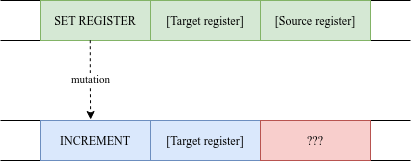
\includegraphics[scale=0.75]{binary_mutation}
    \caption{Mutating the first byte of a three-byte instruction can turn it into a two-byte instruction, leaving one byte to change the meaning of bytes after it.}
\end{figure}

Using linear programs for genetic programming is not impossible, and it has been done to great success in the past. However, the extra complexity that this would introduce was something I wanted to avoid. As such, I opted to instead use tree-based programs, something which is more natural to functional programming than imperative programming. Still, converting a tree to an imperative program is not difficult, and trees would be much easier to work with for the genetic algorithm.

\subsection{Structure}
The tree-based programs are constructed using nodes, which can have a function or value and, depending on their arity, a number of children. The types of nodes implemented are as follows:

\begin{minted}{rust}
pub enum Node {
    Null,
    Val(Source),
    Unary(UnaryOperation, Box<Node>),
    Binary(BinaryOperation, Box<Node>, Box<Node>),
    Then(Box<Node>, Box<Node>),
    Print(Box<Node>),
    Store(Reg, Box<Node>),
    /// condition, if_not_zero, if_zero
    If(Box<Node>, Box<Node>, Box<Node>),
    /// condition, block; repeat block until condition equals zero
    While(Box<Node>, Box<Node>),
    /// count, block; repeat block count times
    Repeat(Box<Node>, Box<Node>),
    Compare(Box<Node>, Box<Node>),
    Turtle(TurtleOperation),
}
\end{minted}

I will also be representing these trees graphically, to aid in their understanding for the purposes of this thesis. For example, the following literal is equivalent to the image below it:
\begin{minted}{rust}
Binary(
    BinaryOperation::Add,
    Box::from(Binary(
        BinaryOperation::Add,
        Box::from(Val(Source::Value(1))),
        Box::from(Val(Source::Value(2))),
    )),
    Box::from(Binary(
        BinaryOperation::Multiply,
        Box::from(Val(Source::Value(3))),
        Box::from(Val(Source::Value(4))),
    )),
)
\end{minted}

\begin{figure}[h]
    \centering
    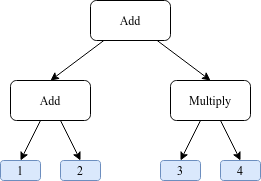
\includegraphics[scale=0.75]{tree_1}
    \caption{A simple tree-based program}
\end{figure}

Since the purpose of these programs is to build structures, they must allow for side effects. To this purpose, the full instruction set is as follows:
\begin{itemize}
    \item \verb|Null|: do nothing.
    \item \verb|Val|: supply a value, either from a register or directly.
    \item \verb|Unary| and \verb|Binary|: execute an operation, using its children as parameters.
    \item \verb|Then|: execute the left child, followed by the right one.
    \item \verb|Print|: print the value of its child returning it, used for debugging.
    \item \verb|Store|: store the value of its child in the given register.
    \item \verb|If|: depending on the value of its leftmost child, execute and return the value of either its middle child or the right one.
    \item \verb|While|: while its left child has a value different from $0$, execute the right one, returning its value on the last iteration. 
    \item \verb|Repeat|: repeat its right child as many times as the value of the left child.
    \item \verb|Compare|: compare the left and right children, returning the comparison result.
    \item \verb|Turtle|: execute a turtle operation and return its result.
\end{itemize}

When mutating a tree is required, it is possible to change out a node for one of the same arity, or even for a completely new subtree, and still have a functioning program.

\begin{figure}[h]
    \centering
    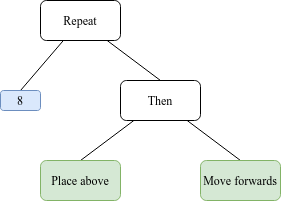
\includegraphics[scale=0.75]{tree_2}
    \caption{A simple program that builds a line from $(0, 1, 0)$ to $(7, 1, 0)$.}
\end{figure}

\subsection{Translation}
The end-goal, as before, is to generate a linear program. This means that a mechanism to convert a tree-based program into a linear one is required.

There are some subtleties to be aware of: the trees are not entirely functional (side effects complicate things), and their code has to be translated into the linear structured described before. The mechanism chosen for this is by making use of a \emph{stack pointer}. This is a variable that holds a reference to a certain register during the translation process, starting with \verb|STACK_START| (100). This variable is incremented when recursing deeper into the tree, and is used to identify the register that should be used for storing the result returned by a subtree. Henceforth, the register referred to by this pointer shall be denoted \verb|r[stack_ptr]|.

Additionally, \emph{labels} are used for control-flow structures. A label is a (linear) instruction holding an unsigned 16-bit integer, used by jump instructions as a target. Every new label instruction receives a new integer, guaranteeing their uniqueness.

Translation follows the following mechanism, where \verb|translate_subtree| is a recursive function:

\begin{minted}{rust}
pub fn translate_tree(tree: &Node) -> Vec<Instruction> {
    let mut next_label = 0u16;
    translate_subtree(tree, STACK_START, &mut next_label)
}

fn translate_subtree(tree: &Node, stack_ptr: u8, next_label: &mut u16) -> Vec<Instruction> {
    match tree {
        ...
    }
}
\end{minted}

For example, a subtree rooted in a unary operation is translated from its children first. Afterwards, the operation is executed on \verb|r[stack_ptr]|, which will have been set to the result of the child subtree.

\begin{minted}{rust}
Node::Unary(op, child) => {
    // do the subtree, which stores result in r[stack_ptr]
    let mut instr = translate_subtree(child, stack_ptr, next_label);
    // do op on r[stack_ptr]
    instr.push(Instruction::Unary(stack_ptr, *op));

    instr
}
\end{minted}

For multiple subtrees, the stack pointer is incremented, so that two separate values may be used:

\begin{minted}{rust}
Node::Binary(op, left, right) => {
    // do left subtree, which stores result in r[stack_ptr]
    let mut instr = translate_subtree(left, stack_ptr, next_label);
    // do right subtree, which stores result in r[stack_ptr + 1]
    instr.append(&mut translate_subtree(right, stack_ptr + 1, next_label));
    // do op on r[stack_ptr] with r[stack_ptr + 1]
    instr.push(Instruction::Binary(stack_ptr, Source::Register(stack_ptr + 1), *op));

    instr
}
\end{minted}

A \verb|Then| node simply adds the instructions for one subtree before the other:

\begin{minted}{rust}
Node::Then(left, right) => {
    // do left subtree, which stores result in r[stack_ptr]
    let mut instr = translate_subtree(left, stack_ptr, next_label);
    // do right subtree, which stores result in r[stack_ptr]
    instr.append(&mut translate_subtree(right, stack_ptr, next_label));

    instr
}
\end{minted}

Conditional nodes, such as \verb|If|, also make use of labels:

\begin{minted}{rust}
Node::If(cond, if_not_zero, if_zero) => {
    let label_else = *next_label;
    let label_after = label_else + 1;
    *next_label += 2;
    // process cond subtree, store result in r[stack_ptr]
    let mut instr = translate_subtree(cond, stack_ptr, next_label);

    // if cond != 0, keep going to the if_not_zero block, then jump to label_after
    instr.push(Instruction::Jump(label_else, JumpCondition::Zero(stack_ptr)));
    instr.append(&mut translate_subtree(if_not_zero, stack_ptr, next_label));
    instr.push(Instruction::Jump(label_after, JumpCondition::None));
    // else, jump to label_else, do the if_zero block, then continue to label_after
    instr.push(Instruction::Label(label_else));
    instr.append(&mut translate_subtree(if_zero, stack_ptr, next_label));
    instr.push(Instruction::Label(label_after));

    instr
}
\end{minted}

Finally, nodes making use of special registers such as the \verb|RESULT_REGISTER| and the \verb|COMPARE_REGISTER| will move results to \verb|r[stack_ptr]| to make them accessible by their parents.

\begin{minted}{rust}
Node::Turtle(operation) => {
    vec!(
        // do the operation, storing result in r[RESULT_REGISTER]
        Instruction::Turtle(*operation),
        // copy r[RESULT_REGISTER] into r[stack_ptr] to move it up the tree
        Instruction::Binary(stack_ptr, Source::Register(RESULT_REGISTER), Set),
    )
}
\end{minted}

For example, the tree below translates into the instructions below it.

\begin{figure}[h]
    \centering
    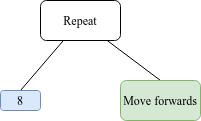
\includegraphics{tree_3}
    \caption{A simple tree.}
\end{figure}

\begin{figure}[h]
\begin{minted}{rust}
Binary(101, Value(8), Set),  // set reg. 101 to 8
Label(0),
Jump(1, Zero(101)),  // jump to label 1 when reg. 101 is 0
Turtle(Move(Forward)),
Binary(100, Register(200), Set),  // set reg. 100 to the value of the result register
Unary(101, Decrement),  // decrement reg. 101
Jump(0, None),  // jump to label 0 always
Label(1)
\end{minted}
\caption{The equivalent list of instructions.}
\end{figure}

\section{Genetic algorithm}

For a brief summary, a genetic algorithm is an algorithm taking inspiration from the real-life processes of natural selection and evolution. It involves taking an entire ``population'' of ``individuals'', in this case tree-structured programs, and evaluating them. The next generation is created from the current one, with individuals that performed better having a higher chance of ``reproducing''. To make helpful changes, individuals are mixed together and randomly modified individually. Here is a short glossary to help with the following section:

\begin{itemize}
    \item \emph{population} or \emph{generation}: a group of individuals evaluated, modified and propagated in a single iteration of the genetic algorithm
    \item \emph{individual}: a single tree, in a population
    \item \emph{evaluation}: the process of checking the performance of every individual in a generation
    \item \emph{fitness}: the weight allocated to each individual during the selection process
    \item \emph{selection}: the process of building a new population from the old one, by copying individuals or crossing them together
    \item \emph{crossover}: the building of one individual out of parts of two parents
    \item \emph{mutation}: using randomness to modify parts of an individual in hope of creating useful new traits
\end{itemize}

The over-all training function, that goes through the generations gradually improving individuals, is detailed below. This function takes as parameter a \verb|target| that the trained individuals are supposed to build.

\begin{minted}{rust}
pub fn train(target: &BlockSpace) -> definitions::Individual {
    // randomly-generate the first generation
    let mut generation = Generation::random();
    // evaluate the first generation
    generation.evaluate(target);
    let mut best_overall = generation.population[0].clone();
    for _gen in 0..GEN_COUNT {
        // find and store the best individual from each generation
        let best_individual = &generation.population[generation.best_index.unwrap()];
        let best_result = &best_individual.result.unwrap();
        // store this individual if it is the best over-all
        if best_result.score > best_overall.result.unwrap().score {
            best_overall = best_individual.clone();
        }
        // select individuals from the current generation to either take part in the next 
        // one directly or as parents for new children
        let (kept_over, parent_pairs) = generation.select_weighted_by_fitness();
        // build a new generation from the selected individuals
        generation = Generation::from_old(&generation, &kept_over, &parent_pairs);
        // produce random, potentially useful mutations in the individuals
        generation.mutate();
        // evaluate the built generation, for the next iteration
        generation.evaluate(target);
    }

    // return the best individual found in any generation
    best_overall
}
\end{minted}

In the following sub-sections, I will go into more detail concerning each part of this algorithm.

\subsection{Creating the first generation}

The first generation is constructed by randomly-generating individuals using two methods and several depths. This method, proposed by J.R. Koza \cite{koza}, is called ``ramped half-and-half''.

The first method is called \emph{full}, and involves creating a full tree down to a certain depth. Nodes below that depth must have a non-zero arity (i.e. not be leaves), and the entire maximum depth must be made up of leaves. The second method, \emph{grow}, permits leaves further up in the tree with a certain probability.

\begin{minted}{rust}
pub fn generate(method: Method, max_depth: usize) -> Node {
    recurse(method, max_depth, 0)
}

fn recurse(method: Method, max_depth: usize, current_depth: usize) -> Node {
    let mut rng = rand::thread_rng();

    if current_depth == max_depth || (method == Method::Grow && rng.gen_bool(P_GROW_LEAF)) {
        // generate a leaf, excluding useless leaves such as the Null node
        random_useful_leaf()
    } else {
        // generate a function, continuing recursion with its children
        random_function(method, max_depth, current_depth)
    }
}
\end{minted}

One useful nuance here is that, even though there exist many types of unary and binary operations, the \verb|Unary| and \verb|Binary| nodes have the same chance to be generated as control structures like \verb|Repeat|. This should, in theory, make it so that programs have a higher chance of generating the comparatively complex structures required to construct parts of structures.

The first generation is constructed using equal numbers of individuals generated using either method, and by varying the \verb|max_depth| parameter between two thresholds (hence the `ramped' part of the name). This results in a nice variety of small and large, simple and complex trees, hopefully providing a relatively unbiased start.

\subsection{Evaluation}

Trees are evaluated against a target structure, measuring how close the built structure is to the target. This measurement is done using the \emph{Sørensen–Dice coefficient}\cite{sorensen}\cite{dice}, henceforth referred to as the ``Dice index''. This index is calculated as follows:

$$DSC = \frac{2TP}{2TP + FP + FN}$$
\begin{align*}\quad
    \text{where}\quad
    TP &= \text{number of true positives}\\
    FP &= \text{number of false positives}\\
    FN &= \text{number of false negatives}
\end{align*}

To be more explicit, a ``true positive'' in this case means a position that is filled in both the target structure and the built one (and similar for the other two terms). This index has a value of $0$ when the two have nothing in common, and $1$ when they are identical (hence, $FP$ and $FN$ are $0$).

One thing that must be taken into account, however, is that a smaller program (shallower tree) should score better than a bigger one (deeper tree) which does the same thing. For this purpose, the actual score of a tree is the following:

$$s = DSC * \frac{DS + MD - d}{DS + MD}$$
\begin{align*}\quad
    \text{where}\quad
    DSC &= \text{Dice index}\\
    DS &= \text{depth softener}\\
    MD &= \text{the maximum allowed depth of a tree}\\\
    d &= \text{the depth of the tree}
\end{align*}

The \emph{depth softener} is a parameter of the algorithm  used to control the importance of tree's depth to the score of an individual; a bigger $DS$ means that depth has less of an impact.

Individuals whose tree exceeds the allowed depth, or whose program either takes too long or terminates with an error, receive a score of $-\infty$.

The \verb|result| field of each individual is made up of its \verb|score|, its unmodified \verb|dice_index|, and a boolean value \verb|perfect| which is set to true if it has a Dice index of 1.

After evaluating each individual, a generation will also store the best score of any individual in the population, as well as the worst finite score found.

\subsection{Selection}

Selection is the process of picking individuals from the current generation to use in the creation of the next one. These individuals are chosen based on their score in one of two ways.

\emph{Tournament selection} involves running a number ``tournaments'' and picking the winner as a parent for the next generation. A tournament involves randomly selecting a handful of individuals from the population, and sorting them by their results. Then, the best individual in this set is chosen with probability $p$, the second with probability $(1-p)p$, etc. If no other individual is chosen, the worst one will be.

Tournament selection only picks parents, so the entirety of the next population will be constructed using crossover.

\emph{Fitness-weighted selection}, on the other hand, is done on the whole population at once. First, each individual's score $s$ is mapped into a fitness $f$ using the following formula:

$$f = \left(\frac{s - s_{min}}{s_{max} - s_{min}}\right)^{SP}$$
\begin{align*}\quad
    \text{where}\quad
    s_{min} &= \text{the worst score in the generation}\\
    s_{max} &= \text{the best\footnotemark score in the generation}\\
    SP &= \text{selection pressure}
\end{align*}

\footnotetext{If every individual in the generation has the same score, then $s_{max}$ will be equal to $s_{min} + 0.1$ instead, in order to avoid division by zero.}

The selection pressure is a parameter that dictates how strongly the selection process is weighed in favor of better individuals.

After the fitness of each individual is calculated, the function uses them as weights to randomly pick (with replacement) a number of individuals from the population to either be copied directly to the next generation, or to serve as parents during the crossover process.

\subsection{Crossover}

To easily explain crossover, both in my code and this sub-section, I will borrow a couple of terms from the field of the horticultural technique of \emph{grafting}, which involves joining tissue from two different plants in order to continue their growth together. In this context, the lower part of the combined plant is called a rootstock or \emph{stock}, while the upper part is called a \emph{scion}. I, however, will be using the two terms to refer to the two trees that will provide the necessary parts, the parents of the new child.

Crossover, for the purposes of genetic algorithms, involves taking two individuals and mixing parts of them together to create a new individual. This is analogous to the real-life genetic process of chromosomal crossover, where matching regions on matching chromosomes break apart and reconnect with each other.

In my code, crossover involves the following process:
\begin{itemize}
    \item pick a weighted-random node of the stock, with leaves having a weight of $1$ and other nodes a weight of $9$, a method again suggested by Koza\cite{koza}
    \item randomly descend the scion to a depth equal to that of the selected node (stopping if a leaf node is hit)
    \item choose a random node from the resulting subtree of the scion, weighing the crossover process in favor of exchanging less genetic material
    \item replace the selected stock node with the chosen node from the scion
\end{itemize}

\begin{minted}{rust}
fn crossover(stock: &Node, scion: &Node) -> Node {
    let mut stock = stock.clone();
    let (stock_point, stock_point_depth) = stock.get_weighted_node_mut();

    // randomly descend as many levels as the stock point is deep, *then* choose a random node
    let scion_point = scion
        .randomly_descend(stock_point_depth)
        .get_weighted_node();

    let mut new_branch = scion_point.clone();
    std::mem::swap(stock_point, &mut new_branch);

    stock
}
\end{minted}

This operation effectively replaces a subtree of the stock with that one of the scion's.

\begin{figure}[h]
    \centering
    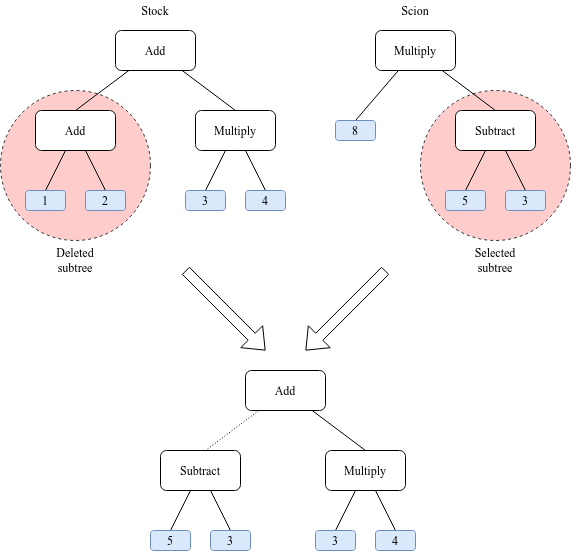
\includegraphics[scale=0.60]{crossover}
    \caption{A stock and a scion combine to produce a single child.}
\end{figure}

\subsection{Mutation}

\chapter{Experiments}

\chapter{Results and conclusions}

\bibliographystyle{abbrv}
\bibliography{bibliography}

\end{document}
